\section{Standard di qualità}\label{section:standard-qualita}

\subsection{Standard ISO/IEC 9126} \label{subsection:9126}
Lo standard ISO/IEC 9126 definisce gli obiettivi qualitativi di prodotto e delinea delle metriche capaci di misurare il raggiungimento di tali obiettivi. Questo standard suddivide in tre aree diverse i criteri qualitativi:
\begin{itemize}
	\item \textbf{Qualità esterna:} è la qualità del prodotto software vista dall'esterno, nel momento in cui esso viene eseguito e testato in un ambiente di prova;
	\item \textbf{Qualità interna:} è la qualità del prodotto software vista dall'interno, ovvero fa riferimento alle caratteristiche implementative del software (architettura e codice);
	\item \textbf{Qualità in uso:} è la qualità del prodotto software vista dall'utilizzatore, il quale ne fa uso all'interno di uno specifico sistema e contesto.
\end{itemize}
È stato deciso di concentrarsi sulla qualità esterna ed interna perchÈ non si ha la possibilità di testare la qualità in uso del prodotto software.\\
Lo standard ISO/IEC 9126 classifica la qualità del software in un insieme strutturato di caratteristiche e sotto-caratteristiche che possono essere misurate quantitativamente attraverso metriche specifiche:
\begin{figure}[H]
	\centering
	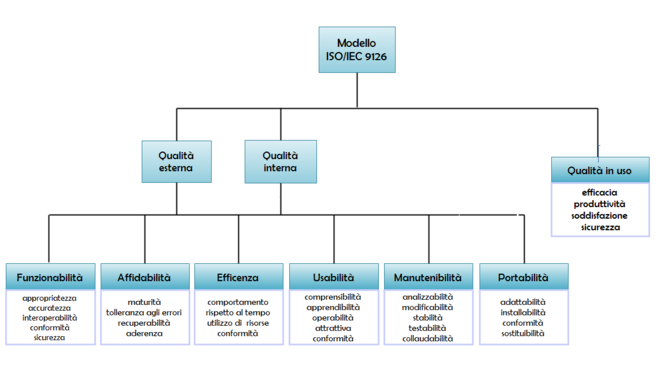
\includegraphics[scale=0.82]{immagini/ISO-IEC_9126.png}
	\caption{Caratteristiche qualitative modello ISO/IEC 9126}
\end{figure}

\begin{itemize}
	\item \textbf{Funzionalità:} capacità del prodotto di fornire funzioni che soddisfano i bisogni impliciti ed espliciti:
	\begin{itemize}
		\item \textbf{Idoneità:} capacità del prodotto di fornire un insieme appropriato di funzioni per attività specifiche;
		\item \textbf{Accuratezza:} capacità del prodotto di fornire risultati corretti o concordati con il gradi di precisione necessario;
		\item \textbf{Interoperabilità:} capacità del prodotto di interagire con uno o più sistemi specifici;
		\item \textbf{Sicurezza:} capacità del prodotto di proteggere i dati e le informazioni in modo da impedire l'accesso e la modifica a persone o sistemi non autorizzati;
		\item \textbf{Conformità funzionale:} capacità del prodotto di aderire a standard, convenzioni o regolamentazioni in materia di funzionalità.
	\end{itemize}
	\item \textbf{Affidabilità:} capacità del prodotto di mantenere un livello di prestazioni adeguato:
	\begin{itemize}
		\item \textbf{Maturità:} capacità del prodotto di evitare fallimenti a causa di errori software;
		\item \textbf{Tolleranza agli errori:} capacità del prodotto di mantenere un livello di prestazioni adeguato anche in caso di errori;
		\item \textbf{Capacità di recupero:} capacità del prodotto di ristabilire le performance ad un livello adeguato e di recuperare i dati in caso di errori;
		\item \textbf{Conformità di affidabilità:} capacità del prodotto di aderire a standard, convenzioni o regolamentazioni in materia di affidabilità.
	\end{itemize}
	\item \textbf{Usabilità:} capacità del prodotto di essere capito e usato dall'utente:
	\begin{itemize}
		\item \textbf{Intelligibilità:} capacità del prodotto di capire se il software è adeguato e come può essere usato per compiti particolari;
		\item \textbf{Apprendibilità:} capacità del prodotto di consentire all'utente di imparare le sue applicazioni;
		\item \textbf{Operabilità:} capacità del prodotto di consentire all'utente di usarlo e controllarlo;
		\item \textbf{Attrattività:} capacità del prodotto di creare interesse nell'utente;
		\item \textbf{Conformità di usabilità:} capacità del prodotto di aderire a standard, convenzioni o regolamentazioni in materia di usabilità.
	\end{itemize}
	\item \textbf{Efficienza:} capacità del prodotto di fornire prestazioni adeguate in relazione alla quantità di risorse usate:
	\begin{itemize}
		\item \textbf{Comportamento temporale:} capacità del prodotto di fornire tempi di risposta e di elaborazione adeguati quando svolge le sue funzioni;
		\item \textbf{Utilizzo di risorse:} capacità del prodotto di tipologia e quantità di risorse adeguate durante la usa esecuzione;
		\item \textbf{Conformità di efficienza:} capacità del prodotto di aderire a standard, convenzioni o regolamentazioni in materia di efficienza.
	\end{itemize}
	\item \textbf{Manutenibilità:} capacità del prodotto di essere modificato, corretto, migliorato e adattato in base ai cambiamenti ambientali, di specifiche o di funzionalità:
	\begin{itemize}
		\item \textbf{Analizzabilità:} capacità del prodotto di poter essere studiato per cercare difetti e carenze;
		\item \textbf{Modificabilità:} capacità del prodotto di consentire l'implementazione di una modifica specifica;
		\item \textbf{Stabilità:} capacità del prodotto di evitare effetti indesiderati causati dalle modifiche;
		\item \textbf{Testabilità:} capacità del prodotto di consentire la validazione di una versione modificata del software;
		\item \textbf{Stabilità:} capacità del prodotto di aderire a standard, convenzioni o regolamentazioni in materia di manutenibilità.
	\end{itemize}
	\item \textbf{Portabilità:} capacità del prodotto di essere trasferito da un ambiente di lavoro ad un altro:
	\begin{itemize}
		\item \textbf{Adattabilità:} capacità del prodotto di essere adattato a diversi ambienti senza la necessità di effettuare modifiche diverse da quelle fornite;
		\item \textbf{Installabilità:} capacità del prodotto di essere installato in specifici ambienti;
		\item \textbf{Coesistenza:} capacità del prodotto di coesistere in ambienti comuni con altri software indipendenti condividendo risorse comuni;
		\item \textbf{Sostituibilità:} capacità del prodotto di sostituire un software analogo con la stessa funzionalità e nello stesso ambiente;
		\item \textbf{Stabilità:} capacità del prodotto di aderire a standard, convenzioni o regolamentazioni in materia di portabilità.
	\end{itemize}
\end{itemize}
\pagebreak
\subsection{Standard ISO/IEC 15504} \label{subsection:ISO/IEC15504}
Lo standard ISO/IEC 15504 definisce come ogni processo debba essere controllato
continuamente al fine di rilevare possibili rischi e debolezze che impediscono il raggiungimento di obiettivi prefissati, e permettono di individuare le possibili cause in modo da migliorare l'efficacia e l'efficienza di tali processi. \\
Il modello SPICE definisce 6 possibili livelli di maturità del processo, ciascuno dotato di attributi utili per misurarla:
\noindent \begin{enumerate}
	\setcounter{enumi}{-1} 
	\item \textbf{Incomplete process (Incompleto):} non include nessun tipo di indicatore, indica che un processo non è implementato oppure è fallito, cioè non ha prodotto nessun risultato.
	\item \textbf{Performed process(Eseguito):} il processo è stato implementato e adempie all’obiettivo prefissato. Il relativo attributo di processo è:
	\begin{itemize}
		\item \textbf{Process performance attribute:} è la misura in cui lo scopo del processo è stato raggiunto.
	\end{itemize}
	\item \textbf{Managed process (Gestito):} il processo viene eseguito in modo controllato in base a obiettivi definiti:
	\begin{itemize}
		\item \textbf{Performance management attribute:} è la misura in cui il processo produce risultati in linea con gli obiettivi prefissati;
		\item \textbf{Work product management attribute:} capacità del processo di elaborare un prodotto documentato, controllato e verificato.
	\end{itemize}
	\item \textbf{Established process:(Stabilito)} il processo definito precedentemente è ora implementato tramite processi capaci di realizzare prodotti adatti. I relativi attributi di processo sono:
	\begin{itemize}
		\item \textbf{Process definition attribute:} è la misura in cui il processo raggiunge i risultati prefissati, aderendo ad uno standard di processo;
		\item \textbf{Process resource attribute:} è la misura in cui il processo sfrutta le risorse allocate.
	\end{itemize}
	\item \textbf{Predictable process (Predicibile):} il processo viene eseguito costantemente entro limiti definiti per raggiungere i risultati attesi. I relativi attributi di processo sono:
	\begin{itemize}
		\item \textbf{Measurement attribute:} è la misura in cui sono misurati i risultati ottenuti per assicurare una buona prestazione dei processi al fine di garantire il raggiungimento degli obiettivi prefissati;
		\item \textbf{Process control attribute:} è la misura in cui il processo viene controllato tramite la raccolta, l’analisi e l’uso di misurazioni del prodotto e di processo con il fine di correggere, solo se necessario, la sua esecuzione per il raggiungimento degli obiettivi fissati;
	\end{itemize}
	\item \textbf{Optimizing process(Ottimizzato):} il processo cambia e si adatta dinamicamente per raggiungere gli obiettivi aziendali. I relativi attributi sono:
	\begin{itemize}
		\item \textbf{Continuos improvement attribute:} è la misura in cui i cambiamenti relativi alla gestione, all’esecuzione e alla definizione di processo sono controllati per raggiungere gli obiettivi di business;
		\item \textbf{Process change attribute:} è la misura in cui vengono identificati e implementati i cambiamenti relativi all’esecuzione del processo.
	\end{itemize}
\end{enumerate}
Ogni attributo di processo precedentemente descritto è misurabile e lo standard predispone 4 differenti livelli:
\begin{itemize}
	\item \textbf{N:} non posseduto (0\% - 15\%);
	\item \textbf{P:} parzialmente posseduto (16\% - 50\%);
	\item \textbf{L:} largamente posseduto (51\% - 85\%);
	\item \textbf{C:} completamente posseduto (86\% - 100\%);
\end{itemize}

\pagebreak
\subsection{Ciclo di Deming - PDCA} \label{subsection:PDCA}
Il ciclo PDCA è un approccio che punta al miglioramento continuo dei processi nel corso del loro svolgimento. Esso si sviluppa in cicli iterativi, ciascuno corrispondente all'esecuzione di una iterazione del processo, suddivisi nelle seguenti 4 fasi:
\begin{itemize}
	\item \textbf{Plan:} fase in cui si stabiliscono gli obiettivi e si svolge la pianificazione dell'esecuzione del processo con annessa valutazione dei costi. In questa fase vengono pianificate eventuali modifiche rispetto a come è stata svolta l'esecuzione del processo in iterazioni precedenti, al fine di ottenere un miglioramento;
	\item \textbf{Do:} fase in cui si esegue il processo secondo la pianificazione e si raccolgono i dati su esecuzione e risultati;
	\item \textbf{Check:} fase in cui vengono controllati i risultati ottenuti nella fase Do e confrontati con gli obiettivi previsti nella fase Plan. In questa fase si valuta se le modifiche effettuate nell'iterazione corrente, non contemplate nelle iterazioni precedenti, hanno portato a miglioramenti della qualità del processo. In questo caso si valuta come rendere standardizzato il processo con tali migliorie apportate;
	\item \textbf{Act:} fase in cui si mette in pratica la standardizzazione delle modifiche migliorative rilevate nell'iterazione corrente. Ciò porta al miglioramento delle iterazioni successive del processo.
\end{itemize}
L'applicazione di questo approccio ciclico in modo continuo sui processi porta al loro miglioramento.

\begin{figure}[H]
	\centering
	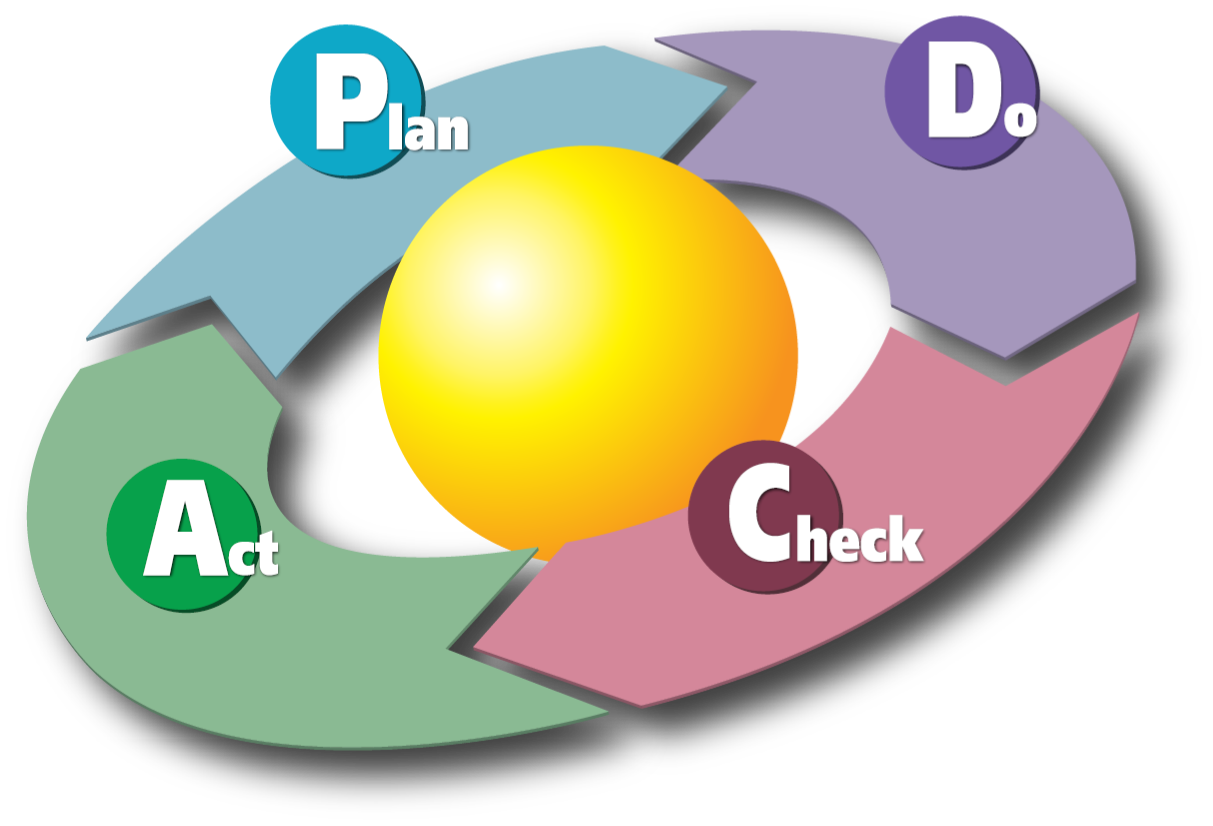
\includegraphics[scale=0.2]{immagini/PDCA.png}
	\caption{Ciclo PDCA}
\end{figure}